\section{Stand der Forschung}


Die zunehmende Tendenz in Deutschland von bargeldlose Bezahlung erfordert neuen Umgang mit den 
eigegebenen Daten. Eine Studie von 2009 der Deutschen Bundesbank zeigte die rasante Anstieg von 
bargeldlose Bezahlung in der Bundesrepublik seit der Einführung von solcher Zahlungsmethode 
\cite{refrep:DBCP}.

\begin{figure}[htb]
    \centering{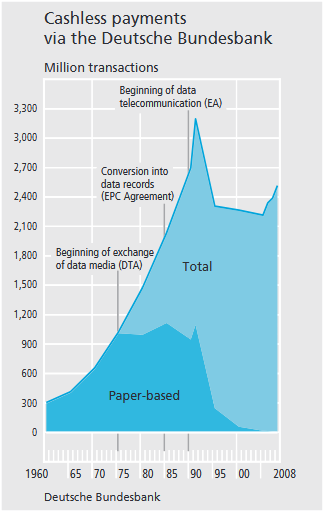
\includegraphics[width=5cm]{Bilder/refrep_DB.png}}
    \caption{Cashless payments via the Deutsche Bundesbank\\ (Bundesbank, 2009, S.52)}
    \label{fig:refrep_DB}
\end{figure}


Laut einer Statistik des Handelsforschungsinstituts EHI von 2019 \cite{refart:KSDL} bezahlen 48,6\% 
der deutschen ihre Waren mit Karte, wohingegen nur noch 46,9\% der deutschen den klassischen 
Weg mit Bargeld gehen. Auch das kontaklose Bezahlen, bei dem bei kleinen Beträgen nicht einmal eine
PIN gefordert wird, nimmt immer weiter zu. Doch gerade bei dieser Variante ist es sehr einfach
im Namen eines anderen zu bezahlen, was eine Sicherheitsrisiko darstellt.


Immer wenn mit Karte bezahlt wird, gehen die Kunden davon aus, dass die Zahlungsabwicklung sicher ist. 
Wie sicher ist das bargeldlose Zahlen heutzutage wirklich? 


Aus diesem Grund ist Vertraulichkeit die erste und wichtigste Voraussetzung, dass ein solches System 
erfüllen muss, um neue potenzielle Kunden zu gewinnen. Unter diesem Begriff soll ein System nur auf 
autorisierte Informationen zugreifen \cite{refbook:SWIS}. In dieser Hinsicht ist die Entwicklung 
einer Click and Buy Maschine so zu konzipieren, dass sie einen sicheren Umgang mit den Kundendaten
anbietet. Diese Interaktion zwischen Kunde und systemkritischen Mechanismen wurde von 
\cite{refart:HARE} so dargestellt:

\vfill
\begin{figure}[htb]
    \centering{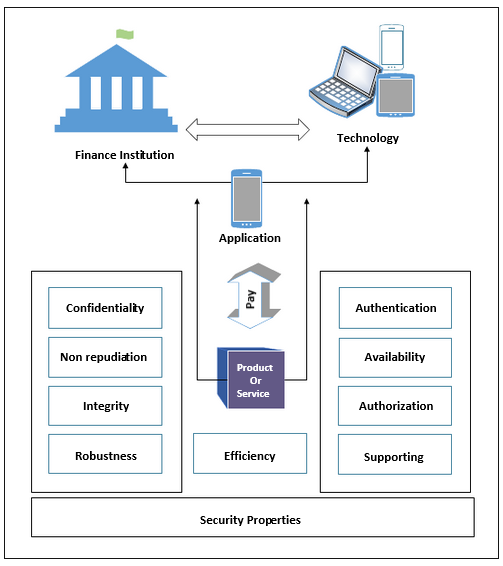
\includegraphics[width=5cm]{Bilder/refark_HARE.png}}
    \caption{Sicherheitseigenschaften von digitalen Zahlungsmethode (Hassan et al. 2020, S8)}
    \label{fig:refark_HARE}
\end{figure}
\vfill

Außerdem sollen die anderen Schutzziele der IT-Sicherheit: Integrität, Verfügbarkeit und
Authentifizierung auch berücksichtg werden, so dass die Systemen einwandfrei funktionieren können.
Eine Zahlungsmethode, bei der alle Vorraussetzungen erfüllt werden, kann in der Lage sein, das Vertrauen und 
die Akzeptanz von den Nutzenden zu bekommen \cite{refart:HARE}. 


\cite{inbook:MHNS} nennt solche Maschinen Cyber-Physical System (CPS), weil sie eine Interaktion zwischen 
Nutzer und einem oder vielen Systemen darstellt. In dieser Zusammenarbeit spielt der Datenaustausch 
eine wesentliche Rolle, besonders von der Seite der Nutzenden. Diese Technologie zielt eine günstigere 
Entwicklung, ohne die Sicherheit zu vernachlässigen. Diese Interaktion findet erfolgereich statt, 
wenn die genannten Sicherheitszielle erfüllt werden.


Da es um einen dynamischen Sektor geht, wo die Änderungen sehr schnell stattfinden, \cite{refip:NYRS} 
muss die Technologie stets weiterentwickelt und angepasst werden, um Vertraulichkeitverlust von seitens
der Kunden zu vermeiden. Dieser Mangel an Vertraulichkt ist das größte Hindernis, warum viele Kunden sich 
verweigern, auf diese Zahlungsmethode zuzugreifen.

\textbf{\textcolor{red}{Ab hier können wir dann versuchen, die Informatien aus den Artikeln zu nehmen, solche
die du hier hinzugefügt hast und solche, die ich dir am Fr schickte}}

\subsection{Drahtlose Verbindungen und Sicherheit bei Bezahlungen}

Viele digitale Zahlungen finden über WLAN statt, das kann eine großere Risiko darstellen \cite{refip:NYRS}, 
da WLAN-Verbindungen als unsicher als normale Kabelverbindungen gilt. Maßnahmen zu entwickeln, die sich an 
verschiedenen Systemen anpassen, kosten Zeit und Investitionen von Banken und Sicherheitsfirmen. Für jeden 
möglichen Angriffe sollen Maßnahmen zur Verfügung gestellt werden, so dass die Integrität des Kunden
geschützt bleibt. Die folgenden Schwachstellen bei digitaler Zahlung wurden von \cite{refip:NYRS} 
zusammengefasst:

\begin{itemize}
    \item Erstellung von Dateien in dem Opfersystem mit umfangreichen Privillegen;
    \item Unzureichende Sicherheit bei der Validierung von Zertifikaten;
    \item Öffentlichkeit des Quellcodes, sodass das System Opfer von Reverse Engineering gezielt ist.
    \item Unsicherer Umgang mit Cookies-Einstellungen
\end{itemize}

\cite{refip:NYRS} schlägt einige Sicherheitsmechanismen vor, die die oben gennanten Schwachstellen bei 
kabelosen Verbindungen vermindern können. Unter denen wird folgende hervorgehoben: 

\begin{itemize}
    \item Nutzung von modernen kryptographischen Standards für die Validierung von Zertifikaten;
    \item Erstellung von Loggdatei, sodass jeder Anormalität schnell überprüft werden kann;
    \item Zwei-Faktor-Authentisierung;
    \item Digitaler und zufällige geordnete Tastatur;
    \item Schwierigkeitsgrad bei der Erstellung von Passwörter;
    \item Besserer Umgang mit der Verwaltung von Cookies;
    \item Registrierung von Geräten;
    \item Künstliche Intelligenz (KI) für die Detektion von abnormalen Verhalten;
    \item Ständig Kontroll gegen Social Engineering.
\end{itemize}

Da drahtlose Zahlungen bei Campingplätzen eine wesentliche Rolle spielen kann, muss die Sicherheit solcher
Zahlungsart gewährleistet werden. Das kann erfolgreich passieren, wenn Banken und andere finanziellen 
Institutionen sich intensiv mit den verschiedenen Angriffsmöglichkeiten und deren Schutzmaßnahmen beschäftigen.

Zahlungskarte wie Kredit- oder EC-Karte sollen auch Zahlungsoptionen von einem Click and Buy Maschinen
zur Verfügung gestellt werden. In Bezug auf diese Modalitäten werden die verschiedenen Aspekten der 
Sicherheit dieser Zahlungsart unter beschrieben.


\subsection{Anwendung von Smartcards und sicheres Bezahlen}
Der Begriff Smartcards bezeichnet eine Plastikkarte mit einem eingebauten Chip, der ein eigenes Betriebssystem,
einen Mikroprozessor und minimale Funktionalitäten besitzt. Sie wurde vor mehr als 40 Jahre erfunden und deren 
Ziel ist die Sicherheit von Kartenzahlung und allgemeine Authentifizierungsverfahren zu erhöhen \cite{refip:JFSB}.
Sie unterscheiden sich von traditionelen Magnetstreifenkarten, weil sie verschiedene Authentifizierungsmethode
ermöglichen auch ohne direkte Verbindung mit der Bank funktionieren könnne \cite{refbook:ATMS}. Ein Abbildung, 
wie das Authentifizierungsprozess von Smartcards funktionier wird unter dargestellt:

\vfill
\begin{figure}[htb]
    \centering{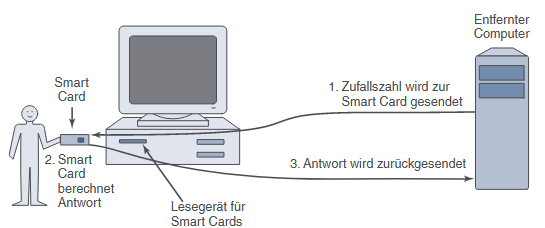
\includegraphics[width=10cm]{Bilder/refbook_ATMS.png}}
    \caption{Authentifizierungsprozess von Smartcards\\(Tanenbaum, 2009, S.755)}
    \label{fig:refbook_ATMS}
\end{figure}
\vfill






: Speicherung, Überprüfung, funktionierende System
auch wenn es keine  eigene Energieversorgung
die 140 Byte Informationen beinhalten und deren Funktion lediglich zur Identitäts- und Pinüberprüfung dient. 
Da 



\textbf{\textcolor{red}{Ich habe Teil des Artikels sehr schnell gelesen. Ich denke, wir können dessen Inhalt hier
irgendwie zusammenfassen. In diesem Fall sprechen wir dann über verschiedene Sicherheitsrisiken und Gegenmechanismus
zuerst für WLAN dann mit Karte usw. \cite{refmas:ASSS}}}

\textbf{\textcolor{red}{Ich würde so machen:}}



\begin{enumerate}
    \item \textbf{\textcolor{red}{Worum es geht, was sind diese Karte}}
    \item \textbf{\textcolor{red}{Sicherheitslücken}}
    \item \textbf{\textcolor{red}{Sicherheitsmechanismen}}
\end{enumerate}

\textbf{Was sind Smartcards}
\begin{enumerate}
    \item \textbf{\textcolor{red}{Hier müssen wir recherchieren. Über was sie sind, würde ich in einer anderen QUelle Schutzmaßnahmen}}
    \item \textbf{\textcolor{red}{Wo werden sie bentutzt. }}
    \item \textbf{\textcolor{red}{Authentifizierung: PIN, CHIP, Mehrfachautentifzierung}}
    \item \textbf{\textcolor{red}{Auch ohne Pin für kleinen Beitra}}
    \item \textbf{\textcolor{red}{kurze beschreibung von Angriffetechnick: Protokollanalyse, Relay   Hardware Reverse Engineering, Angriffebeispiel: legic prime, mifare  }}
    \item \textbf{\textcolor{red}{Gegenmassnahmen: physikalisch, logisch: authentifzierung, besserere verschlüssung. Andere Quelle suchen }}
\end{enumerate}


\vfill
\begin{figure}[htb]
    \centering{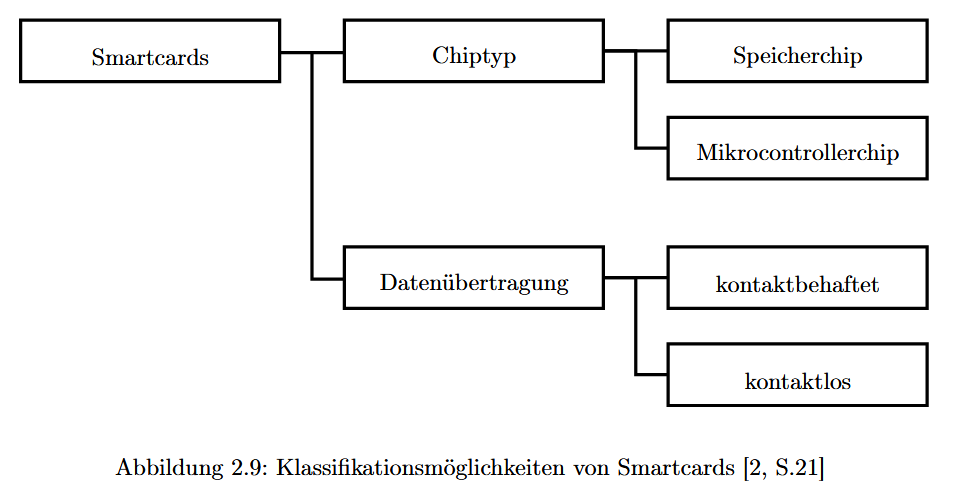
\includegraphics[width=5cm]{Bilder/refmas_ASSS.png}}
    \caption{Abbildung von Smartcards - Das kann später verbessert werden}
    \label{fig:refmas:ASSS}
\end{figure}
\vfill



\vspace{2cm}
\textbf{Ich würde diesen Satz in den nächsten Kapitel verwenden und erweitern mit unseren Recherchen, damit wird 
die Literatur rechtfertigen können}
Um das zu bewerkstelligen, ist der aktuelle technische Stand von entscheidener Bedeutung. 
Ausgehend von dieser Informationen muss das Glasfasernetz eventuell erweitert oder auch neu verlegt werden.
Denn das Ziel ist es, technisch gesehen auf dem neusten Stand zu sein, damit das Click and Buy System für die Zukunft abgesichert ist.
Außerdem wird durch den Ausbau des Glasfasernetzes die Region insgesamt deutlich attraktiver gemacht, was vielleicht auch Menschen dazu bringt
in diese Region zu ziehen. Denn jedem ist klar, dass ein guter Internetausbau essentiell ist, um vielleicht auch mal von zuhause aus zu arbeiten.